\chapter{Development Environment and Conventions}

In this part, we will see the development environment we used, and the programming conventions we've applied.

\section{Development Environment}

\subsection{GitHub}

To write this report and to be able to implement both models most effectively possible, we used a tool of hosting and management of program which is called Github. It is a tools of versionning which allows the collaborative work and allows a simplification of the methods of work.\\
We used it throughout the project to put the summaries of articles that we read, the result og our meeting, this report or still implementations.\\
Our Git repository is located at the following address : \\
\url{https://github.com/jetcheve/M2\_PER\_MMUAVGRA}.\\

Our deposit is decomposes into three branches :

\begin{itemize}
\item A master branch which is general to the whole deposit.
\item A branch called Develop. It's in this branch that there will be all the code for implementing different models.
\item An branch report, which as its name suggests, contain all the parts of our report and his pictures.
\end{itemize}

\subsection{Eclipse}

Eclipse is an integrated development environment for creating projects in any programming language. It is used to develop programs in JAVA, Android, C, etc.\\

We used Eclipse throughout the project implementation.\\

As a supplement to Eclipse, we used a library that is called JBotsim \cite{JBotSim} proposed by Mr. Casteigts. This allows to simulate a dynamic network. This network is simulated with mobile nodes that interact. These nodes can send messages (in our case, maps of each UAVs).\\

We used this library because it is very easy to use, and it adapt well to the needs which we had.

\section{Programming Conventions}

First, we've choosed to used the Java Coding Conventions, which we can see in the following link \url{http://www.oracle.com/technetwork/java/codeconventions-150003.pdf}\\

Then, in order to create our documentation, we've used the Doxygen Convention, viewable here \url{http://www.stack.nl/~dimitri/doxygen/manual/docblocks.html}\\
We've relied heavily on this documentation and have mostly employed these protocoles below.\\

\lstset{language=Java,basicstyle=\footnotesize,commentstyle=\color{blue}}
\begin{lstlisting}[frame=trBL, title=Doxygen Convention for classes]
/**
* @class name of the class
* @brief Description of herself
*/
\end{lstlisting}

\lstset{language=Java,basicstyle=\footnotesize,commentstyle=\color{blue}}
\begin{lstlisting}[frame=trBL, title=Doxygen Convention for methods]
/**
* @brief Description of the method
* @param the parameters and their descriptions
* @return the description of what return the method (optional)
*/
\end{lstlisting}

\lstset{language=Java,basicstyle=\footnotesize,keywordstyle=\color{red},commentstyle=\color{blue}}
\begin{lstlisting}[frame=trBL, title=Doxygen Convention for members]
int var; /**< Detailed description after the member */
\end{lstlisting}
~\\

We've also resorted to programming conventions that we defined between us.\\
For example, when a part of a code, was not finished yet, we put the following lines above the concerning part.\\\\\\\\

\lstset{language=Java,basicstyle=\footnotesize,commentstyle=\color{blue}}
\begin{lstlisting}[frame=trBL, title=Programming convention for unfinished code]
/**
* @TO_DO
* Description
*/
\end{lstlisting}
~\\

We've also used a convention for the bugs found and wrote these lines.\\

\lstset{language=Java,basicstyle=\footnotesize,commentstyle=\color{blue}}
\begin{lstlisting}[frame=trBL, title=Programming convention for bugs]
/**
* @BUG
* Description
*/
\end{lstlisting}
~\\

We've also used GitHub, in order to manage us.\\
Indeed, it allows us :\\

\begin{itemize}
\item to create tasks, 
\item assign somebody to a task, 
\item see if a task is finish or not,
\item create Milestones, which is a set of tasks to do in a specific time, 
\item and see the state of our progress,
\item define kinds of tasks (development, bug, report ...)
\end{itemize}
~\\

\begin{figure}[!h]
\caption{\label{Milestones}Progress state of Milestones}
   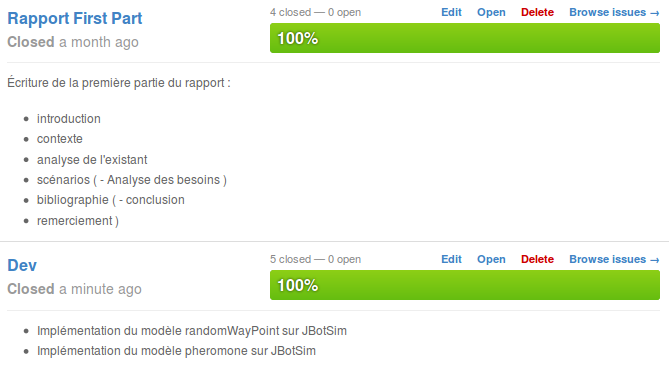
\includegraphics[scale=0.7]{../images/Milestones.png}
\end{figure}

\begin{figure}[!h]
\caption{\label{Tasks}Example of Tasks}
   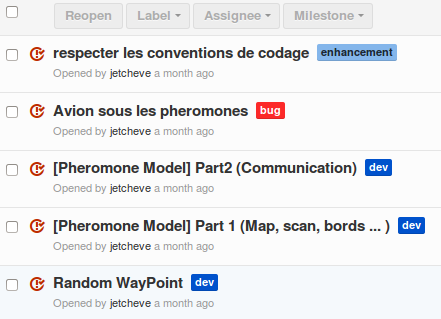
\includegraphics[scale=0.7]{../images/tasks.png}
\end{figure}


To finish, we've created the five essential files for a project :

\begin{itemize}
\item INSTALL.txt  : Installation instructions for the project,
\item LICENCE.txt  : Licence and copyright \copyright{} of the project,
\item README.txt   : General description of the project,
\item AUTHORS.txt  : Authors of the project,
\item MANIFEST.txt : Tree structure and files list of the project.
\end{itemize}
